%%%%%%%%%%%%%%%%%%%%%%%%%%%%%%%%%%%%
% Slide options
%%%%%%%%%%%%%%%%%%%%%%%%%%%%%%%%%%%%

% Option 1: Slides with solutions

\documentclass[slidestop,compress,mathserif]{beamer}
\usepackage{booktabs}
\newcommand{\soln}[1]{\textit{#1}}
\newcommand{\solnGr}[1]{#1}

% Option 2: Handouts without solutions

%\documentclass[11pt,containsverbatim,handout]{beamer}
%\usepackage{booktabs}
%\usepackage{pgfpages}
%\pgfpagesuselayout{4 on 1}[letterpaper,landscape,border shrink=5mm]
%\newcommand{\soln}[1]{ }
%\newcommand{\solnGr}{ }

%%%%%%%%%%%%%%%%%%%%%%%%%%%%%%%%%%%%
% Style
%%%%%%%%%%%%%%%%%%%%%%%%%%%%%%%%%%%%
%%%%%%%%%%%%%%%%%%%%%%%%%%%%%%%%%%%%%%%%%%%%%%%%%%%%%%%%%%%%%%%%%%%%%%%%
% MA213/214 shared slide style
%
% "Calm & Cool" palette + content-type callout boxes.
% Overhauled (2026) from the original OpenIntro/metropolis style:
%   - all OpenIntro visual branding removed (logo, grid, colors)
%   - a low-key cool palette (see colors below)
%   - tcolorbox callout boxes so students recognize content types
% See common/README.md for the command cheat-sheet.
%%%%%%%%%%%%%%%%%%%%%%%%%%%%%%%%%%%%%%%%%%%%%%%%%%%%%%%%%%%%%%%%%%%%%%%%

\usetheme{metropolis}

%%%%%%%%%%%%%%%%
% Packages
%%%%%%%%%%%%%%%%

\usepackage{geometry}
\usepackage{graphicx}
\usepackage{amssymb}
\usepackage{epstopdf}
\usepackage{amsmath}  	% this permits text in eqnarray among other benefits
\usepackage{url}		% produces hyperlinks
\usepackage{hyperref}	% allows for color usage in tables
\usepackage[english]{babel}
\usepackage[latin1]{inputenc}
\usepackage{colortbl}	% allows for color usage in tables
\usepackage{multirow}	% allows for rows that span multiple rows in tables
\usepackage{color}		% this package has a variety of color options
\usepackage{pgf}
\usepackage{calc}
\usepackage{ulem}
\usepackage{multicol}
\usepackage{textcomp}
\usepackage{txfonts}
\usepackage{listings}
\usepackage{tikz}
\usepackage{array}
\usepackage{wasysym}
\usepackage{fancyvrb}
\usepackage{etoolbox}             % \ifstrempty for optional box subtitles
\usepackage[most]{tcolorbox}      % content-type callout boxes
\tcbuselibrary{listings}          % R-code block (\begin{rblock})
\usepackage{fontawesome5}         % box icons

%%%%%%%%%%%%%%%%
% Remove navigation symbols
%%%%%%%%%%%%%%%%

\setbeamertemplate{navigation symbols}{}

%%%%%%%%%%%%%%%%
% "Calm & Cool" palette
%%%%%%%%%%%%%%%%

% chrome / structure / body
\definecolor{ccSlate}{HTML}{2E3742}   % frametitle bar, structure, section pages (deep neutral slate)
\definecolor{ccInk}{HTML}{2B2B2B}     % body text
\definecolor{ccWash}{HTML}{FCF8F1}    % gentle warm title-slide background wash (complements the cool blues)

% example (blue)
\definecolor{ccBlue}{HTML}{2F6690}
\definecolor{ccBlueBg}{HTML}{EAF1F7}
% interactive activity / discussion (green)
\definecolor{ccGreen}{HTML}{4E8A6B}
\definecolor{ccGreenBg}{HTML}{E9F3EC}
% solution (purple)
\definecolor{ccPurple}{HTML}{6F5499}
\definecolor{ccPurpleBg}{HTML}{EFEAF6}
% worksheet / focused work (terracotta)
\definecolor{ccTerra}{HTML}{C2693E}
\definecolor{ccTerraBg}{HTML}{FAEDE4}
% formula / definition (neutral slate)
\definecolor{ccGray}{HTML}{5C6B7A}
\definecolor{ccGrayBg}{HTML}{EEF1F4}
% caution / common pitfall (brick red)
\definecolor{ccRed}{HTML}{B23A48}
\definecolor{ccRedBg}{HTML}{FAEAEC}
% key idea / takeaway (muted gold)
\definecolor{ccGold}{HTML}{9C7A28}
\definecolor{ccGoldBg}{HTML}{F7F1DF}
% learning goals / lesson outcomes (teal)
\definecolor{ccTeal}{HTML}{2C6E6B}
\definecolor{ccTealBg}{HTML}{E6F0EF}
% learning objectives (indigo)
\definecolor{ccIndigo}{HTML}{45507A}
\definecolor{ccIndigoBg}{HTML}{ECEEF4}
% R code / output (gray)
\definecolor{ccCode}{HTML}{5F5E5A}
\definecolor{ccCodeBg}{HTML}{F4F5F6}

% neutral grays kept from the original style
\definecolor{gray}{rgb}{0.5, 0.5, 0.5}
\definecolor{darkGray}{rgb}{0.3, 0.3, 0.3}
\definecolor{darkerGray}{rgb}{0.2, 0.2, 0.2}

% Backwards-compatible aliases: old OpenIntro color names now point at the
% new palette, so existing \textcolor{oiB}{...}, \hl{...}, etc. keep working.
\colorlet{oiB}{ccBlue}
\colorlet{oiG}{ccGreen}
\colorlet{hlblue}{ccBlue}
\colorlet{rubineRed}{ccRed}
\colorlet{irishGreen}{ccGreen}
\colorlet{lightGreen}{ccGreen}

%%%%%%%%%%%%%%%%
% Restyle metropolis with the Calm & Cool chrome
%%%%%%%%%%%%%%%%

\metroset{block=fill}

\setbeamercolor{normal text}{fg=ccInk, bg=white}
\setbeamercolor{structure}{fg=ccSlate}
\setbeamercolor{alerted text}{fg=ccBlue}
\setbeamercolor{example text}{fg=ccGreen}
\setbeamercolor{frametitle}{bg=ccSlate, fg=white}
\setbeamercolor{progress bar}{fg=ccBlue}
\setbeamercolor{title separator}{fg=ccBlue}
\setbeamercolor{title}{fg=ccSlate}
\setbeamercolor{subtitle}{fg=ccBlue}
\setbeamercolor{author}{fg=ccInk}
\setbeamercolor{institute}{fg=ccGray}
\setbeamercolor{date}{fg=ccGray}
\setbeamercolor{section title}{fg=ccSlate}
\setbeamercolor{standout}{fg=white, bg=ccSlate}

% Section pages sit on the same warm wash as the title slide. We keep
% metropolis's section-title styling and just paint a full-page ccWash
% background behind it (needs >=2 pdflatex passes for the current-page node).
\setbeamertemplate{section page}{%
  \begin{tikzpicture}[remember picture, overlay]
    \fill[ccWash] (current page.south west) rectangle (current page.north east);
  \end{tikzpicture}%
  \centering
  \begin{minipage}{22em}
    \raggedright
    \usebeamercolor[fg]{section title}%
    \usebeamerfont{section title}%
    \insertsectionhead\\[-1ex]
    \usebeamertemplate*{progress bar in section page}%
    \par
  \end{minipage}\par
  \vspace{\baselineskip}
}

%%%%%%%%%%%%%%%%
% Custom inline text commands (recolored to the palette)
%%%%%%%%%%%%%%%%

% degree
\newcommand{\degree}{\ensuremath{^\circ}}

% cite
\newcommand{\ct}[1]{
\vfill
{\tiny #1}}

\newcommand{\NamedNote}[2]{
\rule{2.5cm}{0.25pt} \\ \textit{\footnotesize{\textcolor{rubineRed}{#1:} \textcolor{darkerGray}{#2}}}}

% Note
\newcommand{\Note}[1]{
\rule{2.5cm}{0.25pt} \\ \textit{\footnotesize{\textcolor{rubineRed}{Note:} \textcolor{darkerGray}{#1}}}}

% Remember
\newcommand{\Remember}[1]{\textit{\scriptsize{\textcolor{ccTerra}{Remember:} #1}}}

% expected counts
\newcommand{\ex}[1]{\textit{\textcolor{ccBlue}{#1}}}

% red
\newcommand{\red}[1]{\textit{\textcolor{rubineRed}{#1}}}

% pink
\newcommand{\pink}[1]{\textit{\textcolor{rubineRed!90!white!50}{#1}}}

% green
\newcommand{\green}[1]{\textit{\textcolor{irishGreen}{#1}}}

% orange
\newcommand{\orange}[1]{\textit{\textcolor{ccTerra}{#1}}}

% links: webURL, webLink, appLink
\newcommand{\webURL}[1]{\urlstyle{same}{ \textit{\textcolor{darkGray}{\url{#1}}}}}
\newcommand{\webLink}[2]{\href{#1}{\textcolor{darkGray}{{#2}}}}
\newcommand{\appLink}[2]{\href{#1}{\textcolor{white}{{#2}}}}

% mail
\newcommand{\mail}[1]{\href{mailto:#1}{\textit{\textcolor{darkGray}{#1}}}}

% highlighting: hl, hlGr, mathhl
\newcommand{\hl}[1]{\textit{\textcolor{hlblue}{#1}}}
\newcommand{\hlGr}[1]{\textit{\textcolor{lightGreen}{#1}}}
\newcommand{\mathhl}[1]{\textcolor{hlblue}{\ensuremath{#1}}}

%%%%%%%%%%%%%%%%
% Structural helpers (unchanged from the original)
%%%%%%%%%%%%%%%%

% two col: two columns
\newenvironment{twocol}[4]{
\begin{columns}[c]
\column{#1\textwidth}
#3
\column{#2\textwidth}
#4
\end{columns}
}

% slot (for probability calculations)
\newenvironment{slot}[2]{
\begin{array}{c}
\underline{#1} \\
#2
\end{array}
}

% pr: left and right parentheses
\newcommand{\pr}[1]{
\left( #1 \right)
}

% cancel
\newcommand{\cancel}[1]{%
    \tikz[baseline=(tocancel.base)]{
        \node[inner sep=0pt,outer sep=0pt] (tocancel) {#1};
        \draw[red, line width=0.5mm] (tocancel.south west) -- (tocancel.north east);
    }%
}

% removepagenumbers
\newcommand{\removepagenumbers}{%
  \setbeamertemplate{footline}{}
}

% change margin
\newenvironment{changemargin}[2]{%
\begin{list}{}{%
\setlength{\topsep}{0pt}%
\setlength{\leftmargin}{#1}%
\setlength{\rightmargin}{#2}%
\setlength{\listparindent}{\parindent}%
\setlength{\itemindent}{\parindent}%
\setlength{\parsep}{\parskip}%
}%
\item}{\end{list}}

% footnote
\long\def\symbolfootnote[#1]#2{\begingroup%
\def\thefootnote{\fnsymbol{footnote}}\footnote[#1]{#2}\endgroup}

% commands from the book
\newenvironment{data}[1]{\texttt{#1}}{}
\newenvironment{var}[1]{\texttt{#1}}{}
\newenvironment{resp}[1]{\texttt{#1}}{}

%%%%%%%%%%%%%%%%
% Content-type callout boxes (tcolorbox)
%
% Each type has a colored title strip (icon + label) over a light fill.
% Color = content type; the label + icon reinforce it (so the cue does
% not rely on color alone).
%%%%%%%%%%%%%%%%

\tcbset{
  cccallout/.style 2 args={
    enhanced, breakable=false,
    colback=#2, colframe=#1, colbacktitle=#1, coltitle=white,
    fonttitle=\bfseries\footnotesize,
    boxrule=0.6pt, arc=2.5pt, outer arc=2.5pt,
    left=5pt, right=5pt, top=3pt, bottom=3pt, boxsep=2pt,
    toptitle=2pt, bottomtitle=2pt, lefttitle=5pt,
    before skip=5pt, after skip=5pt,
  },
}

% One-off / collection of examples (blue): \workedexample[subtitle]{body}.
% (Named \workedexample, not \example, because beamer defines \example.)
\newtcolorbox{examplebox}[1][]{cccallout={ccBlue}{ccBlueBg},
  title={\faIcon{lightbulb}~~Example\ifstrempty{#1}{}{ \textmd{---}\ #1}}}
\newcommand{\workedexample}[2][]{\begin{examplebox}[#1]#2\end{examplebox}}

% Running-example header (blue): \examplehead{name} at the top of each frame of a
% multi-slide running example. A one-off or a collection of examples uses the
% \workedexample box above instead.
\newcommand{\examplehead}[1]{%
  \vspace{-0.4em}\par\noindent\tcbox[on line, colback=ccBlue, colframe=ccBlue, coltext=white,
    boxrule=0pt, arc=2pt, left=5pt, right=5pt, top=1pt, bottom=1pt,
    box align=base, nobeforeafter]{\footnotesize\bfseries\faIcon{lightbulb}\,Running example}%
  \ifstrempty{#1}{}{\enspace{\footnotesize\bfseries\textcolor{ccBlue}{#1}}}%
  \par\nobreak\vspace{-0.6em}{\color{ccBlue}\rule{\linewidth}{0.7pt}}\par\nobreak\vspace{-0.8em}}

% Interactive activity (green): \activity[subtitle]{body}
\newtcolorbox{activitybox}[1][]{cccallout={ccGreen}{ccGreenBg},
  title={\faIcon{users}~~Activity\ifstrempty{#1}{}{ #1}}}
\newcommand{\activity}[2][]{\begin{activitybox}[#1]#2\end{activitybox}}

% Discussion question (green): \dq{body}
\newtcolorbox{dqbox}{cccallout={ccGreen}{ccGreenBg}, title={\faIcon{comments}~~Discussion}}
\newcommand{\dq}[1]{\begin{dqbox}#1\end{dqbox}}

% Solution (purple): \solnbox{body}. Gated by the per-deck \soln toggle, so it
% shows in the instructor build and vanishes from the student handout build.
% (Named \solnbox, not \solution, because beamer already defines \solution.)
\newtcolorbox{solutionbox}{cccallout={ccPurple}{ccPurpleBg}, title={\faIcon{key}~~Solution}}
\newcommand{\solnbox}[1]{\soln{\begin{solutionbox}#1\end{solutionbox}}}

% Worksheet / focused work (terracotta): \worksheet[subtitle]{body}
\newtcolorbox{worksheetbox}[1][]{cccallout={ccTerra}{ccTerraBg},
  title={\faIcon{pencil-alt}~~Worksheet\ifstrempty{#1}{}{ #1}}}
\newcommand{\worksheet}[2][]{\begin{worksheetbox}[#1]#2\end{worksheetbox}}

% Formula / definition (neutral slate). Supports both real usages found in the
% decks: \formula{title}{body} and the bare \formula{body} (title defaults to
% "Formula"). The second group is an optional brace argument.
\newtcolorbox{formulabox}[1][Formula]{cccallout={ccGray}{ccGrayBg},
  title={\faIcon{square-root-alt}~~#1}}
\NewDocumentCommand{\formula}{m g}{%
  \IfNoValueTF{#2}%
    {\begin{formulabox}#1\end{formulabox}}%
    {\begin{formulabox}[#1]#2\end{formulabox}}}

% Common pitfall / caution (brick red): \caution[subtitle]{body}
\newtcolorbox{cautionbox}[1][]{cccallout={ccRed}{ccRedBg},
  title={\faIcon{exclamation-triangle}~~Caution\ifstrempty{#1}{}{ #1}}}
\newcommand{\caution}[2][]{\begin{cautionbox}[#1]#2\end{cautionbox}}

% Key idea / takeaway (muted gold): \keyidea[subtitle]{body}
\newtcolorbox{keyideabox}[1][]{cccallout={ccGold}{ccGoldBg},
  title={\faIcon{star}~~Key idea\ifstrempty{#1}{}{ #1}}}
\newcommand{\keyidea}[2][]{\begin{keyideabox}[#1]#2\end{keyideabox}}

% Learning goals / lesson outcomes (teal): \goals{body}. Sits under the short
% LO headings on the objectives slide; body is the "you should be able to" list.
\newtcolorbox{goalsbox}{cccallout={ccTeal}{ccTealBg}, fontupper=\footnotesize,
  top=1pt, bottom=2pt, boxsep=1pt, before skip=3pt,
  title={\faIcon{bullseye}~~By the end of today, you should be able to\ldots}}
\newcommand{\goals}[1]{\begin{goalsbox}#1\end{goalsbox}}

% Learning objectives (indigo): \objectives{body} -- the formal LO headings,
% shown alongside \goals on the objectives slide.
\newtcolorbox{objectivesbox}{cccallout={ccIndigo}{ccIndigoBg}, fontupper=\small,
  top=1pt, bottom=2pt, boxsep=1pt, before skip=3pt,
  title={\faIcon{clipboard-list}~~Learning objectives}}
\newcommand{\objectives}[1]{\begin{objectivesbox}#1\end{objectivesbox}}

% Defaults for a bare \begin{lstlisting}. Without these it inherits the listings
% package defaults: 11pt type, fixed-width columns (which spaces code out as
% "a g e _ f i t"), and no line breaking, so a long line silently runs off the
% right edge of the slide. A deck that passes its own basicstyle still wins.
% Layout only -- syntax coloring is left to the \begin{rblock} environment.
\lstset{
  basicstyle=\ttfamily\footnotesize, columns=fullflexible,
  breaklines=true, breakindent=1.5em, showstringspaces=false,
  numbers=none, frame=none}

% R code / output (gray): \begin{rblock}[subtitle] ... \end{rblock}
% NOTE: a frame containing an rblock must be declared \begin{frame}[fragile].
\lstdefinestyle{ccR}{
  language=R, basicstyle=\ttfamily\footnotesize, columns=fullflexible,
  breaklines=true, showstringspaces=false, numbers=none, frame=none,
  keywordstyle=\color{ccBlue}, commentstyle=\color{ccGreen!75!black},
  stringstyle=\color{ccTerra}}
\newtcblisting{rblock}[1][]{cccallout={ccCode}{ccCodeBg},
  title={\faIcon{terminal}~~R\ifstrempty{#1}{}{ #1}},
  listing only, listing style=ccR}

% --- Legacy boxes (kept so existing decks compile) ---

% app: application exercise -> alias of activity
\newcommand{\app}[1]{\activity{#1}}

% pq: practice question (green, interactive family)
\newtcolorbox{pqbox}{cccallout={ccGreen}{ccGreenBg}, title={\faIcon{list-ol}~~Practice}}
\newcommand{\pq}[1]{\begin{pqbox}#1\end{pqbox}}

% solnMult: solutions for multiple-choice practice questions (uses \soln toggle)
\newcommand{\solnMult}[1]{
\item[] \vspace{-0.59cm}
\only<1>{\item #1}
\soln{\only<2->{\item \orange{#1}}}
}

%%%%%%%%%%%%%%%%
% De-branded title frame + attribution
%%%%%%%%%%%%%%%%

% Eyebrow line on the title slide; a deck may \renewcommand this.
\newcommand{\coursetag}{MA214: Applied Statistics}

% Attribution: all slides released under CC BY-SA, crediting both the
% instructor (later material) and OpenIntro (basis of the earlier material).
\newcommand{\courseattribution}{%
  Slides by Jonathan H.~Huggins, building on materials from OpenIntro's
  \emph{Introduction to Modern Statistics} (Mine \c{C}etinkaya-Rundel et al.).
  Released under the
  \webLink{http://creativecommons.org/licenses/by-sa/3.0/us/}{CC BY-SA license}.
  Some images included under fair use (educational purposes).}

% \maketitleframe: de-branded title slide (no logo, no grid). Uses the deck's
% \title, \subtitle, and \coursetag.
\newcommand{\maketitleframe}{%
  \addtocounter{framenumber}{-1}%
  {\removepagenumbers
  \setbeamercolor{background canvas}{bg=ccWash}%
  \begin{frame}[plain]
    \vspace*{2.6em}
    {\color{ccSlate}\rule{\textwidth}{2.5pt}}\par\vspace{1.5em}
    {\usebeamerfont{date}\scshape\color{ccGray}\coursetag}\par\vspace{0.55em}
    {\usebeamerfont{title}\color{ccSlate}\inserttitle\par}
    \vspace{0.45em}{\color{ccBlue}\rule{3em}{2.5pt}}\par\vspace{0.7em}
    {\usebeamerfont{subtitle}\color{ccBlue}\insertsubtitle\par}
    \vfill
    {\color{ccGray!55}\rule{\textwidth}{0.4pt}}\par\vspace{0.45em}
    {\tiny\color{ccGray}\courseattribution\par}
    \vspace*{0.4em}
  \end{frame}}}

%%%%%%%%%%%%%%%%
% Graphics
%%%%%%%%%%%%%%%%

\DeclareGraphicsRule{.tif}{png}{.png}{`convert #1 `dirname #1`/`basename #1 .tif`.png}

\graphicspath{ {../../common/} {figures/} }

% Preamble
\title[Lecture 20]{Lecture 20: Posterior inference \& prediction}
\subtitle{Module 4: Bayesian Statistics}
\author{Jonathan H.~Huggins}
\institute{}
\date{}

\begin{document}

%%%%%%%%%%%%%%%%%%%%%%%%%%%%%%%%%%%%
% Title page
%%%%%%%%%%%%%%%%%%%%%%%%%%%%%%%%%%%%

\maketitleframe

%%%%%%%%%%%%%%%%%%%%%%%%%%%%%%%%%%%%
% Agenda
%%%%%%%%%%%%%%%%%%%%%%%%%%%%%%%%%%%%

% !TEX root =  Lecture20.tex


%%%%%%%%%%%%%%%%%%%%%%%%%%%%%%%%%%%%
% Recap/Agenda
%%%%%%%%%%%%%%%%%%%%%%%%%%%%%%%%%%%%
\begin{frame}
\frametitle{Module 4: Bayesian Statistics}
    \begin{itemize}
        \item \hl{Previously:} grid approximation and MCMC, so we can now get a posterior for any model.
        \item \hl{This time:} we \emph{use} it, for everything Lectures 18 and 19 deferred.
          \begin{itemize}
              \item \hl{point estimates} and \hl{credible intervals}: what ``95\%'' means;
              \item \hl{hypothesis tests}: a claim's probability, read straight off the posterior;
              \item \hl{model comparison}, applying Bayes' rule to models rather than parameters;
              \item \hl{prediction} for a new observation, and \hl{predictive checking}.
          \end{itemize}
        \item \hl{Reading:} Bayes Rules!\ Chapter 8.
        \item \hl{Homework:}
    \end{itemize}
\end{frame}


%%%%%%%%%%%%%%%%%%%%%%%%%%%%%%%%%%%%
% Learning objectives:
%%%%%%%%%%%%%%%%%%%%%%%%%%%%%%%%%%%%
\begin{frame}
    \frametitle{Lecture Objectives}
    \goals{%
    \begin{itemize}
    \item \hl{estimate a parameter} from a posterior, and say how the posterior mean differs from the MLE;
    \item construct a \hl{credible interval}, and say how it differs from a confidence interval;
    \item test a hypothesis as a \hl{posterior tail probability}, summarized by a Bayesian $s$-value;
    \item \hl{compare two models} by turning their priors into posterior probabilities;
    \item build a \hl{posterior predictive} distribution, and see why averaging beats plugging in;
    \item use \hl{predictive checking}: simulate data from the fitted model and compare.
    \end{itemize}}
\end{frame}


%%%%%%%%%%%%%%%%%%%%%%%%%%%%%%%%%%%%
\begin{frame}
    \frametitle{Lecture Objectives}
    \objectives{%
    \begin{itemize}
    \item \textbf{(M4, LO4)} Inference and Prediction: estimate parameters, construct credible intervals, compare models, and make predictions from a posterior
    \end{itemize}}
    \vspace{0.3em}
    {\small Building on, and revisiting:}
    \objectives{%
    \begin{itemize}
    \item \textbf{(M4, LO3)} Conjugate Models: the Beta-Binomial, Normal-Normal, and Gamma-Poisson posteriors from Lecture 18
    \item \textbf{(M4, LO5)} Markov chain Monte Carlo: the posterior draws from Lecture 19, reused here to predict
    \end{itemize}}
\end{frame}


%%%%%%%%%%%%%%%%%%%%%%%%%%%%%%%%%%%%%%%%%%%%%%%%%%%%%%%%%%%%%%%%%%%%%%%%
\begin{frame}
\frametitle{From a glimpse to a definition}

Lecture 18 read an interval off the birthweight posterior and called it a \hl{credible interval}: an interval $\mu$ falls in with probability 0.95, given the data. It answered ``how likely is this claim?'' with a posterior probability rather than a $p$-value.

\pause
\medskip

Both were used without a definition. This lecture supplies them, and adds model comparison, prediction, and a check on whether the model fits.

\pause
\medskip

\keyidea{There is nothing new to compute. Once the posterior is in hand, every one of these is an area under it.}
\end{frame}

%%%%%%%%%%%%%%%%%%%%%%%%%%%%%%%%%%%%%%%%%%%%%%%%%%%%%%%%%%%%%%%%%%%%%%%%
% Section: Point Estimates and Credible Intervals
%%%%%%%%%%%%%%%%%%%%%%%%%%%%%%%%%%%%%%%%%%%%%%%%%%%%%%%%%%%%%%%%%%%%%%%%
\section{Point estimates and credible intervals}

%%%%%%%%%%%%%%%%%%%%%%%%%%%%%%%%%%%%%%%%%%%%%%%%%%%%%%%%%%%%%%%%%%%%%%%%
\begin{frame}
\frametitle{Estimating the parameter}

The posterior is a whole distribution, but often you must report \emph{one number}: its center, the \hl{posterior mean} (median, if skewed). Below, the observed rate is held at $x/n = 1/3$ as $n$ grows.

\begin{center}
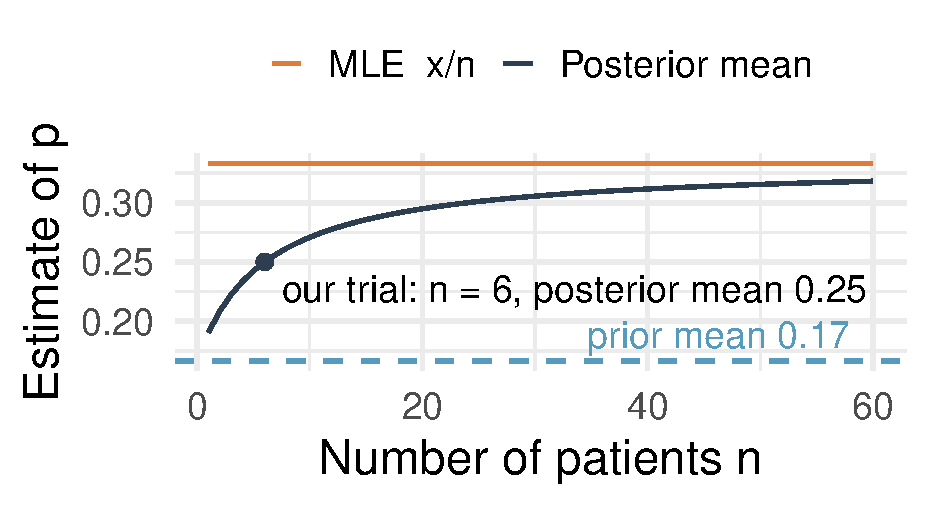
\includegraphics[width=0.62\textwidth]{point_estimate.pdf}
\end{center}

\begin{itemize}
    \item The \hl{MLE} $x/n$ ignores the prior; the \hl{posterior mean} is pulled from it toward the prior mean.
    \item Drug: MLE $0.33$ vs.\ mean $0.25$. Whales: $4.43$ vs.\ $4.11$/day.
\end{itemize}
\end{frame}

%%%%%%%%%%%%%%%%%%%%%%%%%%%%%%%%%%%%%%%%%%%%%%%%%%%%%%%%%%%%%%%%%%%%%%%%
\begin{frame}
\frametitle{Credible intervals}

\formula{Credible interval}{Write $\theta$ for whatever parameter the posterior is over ($p$, $\mu$, $\lambda$, \ldots). A $95\%$ \hl{credible interval} $[a,b]$ satisfies $P(a \le \theta \le b \mid \text{data}) = 0.95$.}

\pause
\medskip

\hl{Interpretation:} given the data we observed, there is a $95\%$ probability that $\theta$ lies in $[a,b]$. A direct statement about the parameter.

\pause
\medskip

\dq{How is this different from a frequentist confidence interval?}

\pause
\medskip

The confidence interval is a statement about the \emph{procedure}: ``if we repeated the study many times, $95\%$ of the intervals would cover $\theta$.'' The credible interval is the interpretation everyone \emph{wishes} a confidence interval had.
\end{frame}

%%%%%%%%%%%%%%%%%%%%%%%%%%%%%%%%%%%%%%%%%%%%%%%%%%%%%%%%%%%%%%%%%%%%%%%%
\begin{frame}
\frametitle{Reading it off the posterior}

The simplest choice is the \hl{equal-tailed} interval: chop $2.5\%$ off each end of the posterior.
\[
a = \text{2.5th percentile}, \qquad b = \text{97.5th percentile of the posterior}.
\]
\pause
\medskip

You already have every tool you need to find those percentiles:
\begin{itemize}
    \item \hl{Conjugate} posterior: read them from the known distribution (\texttt{qbeta}, \texttt{qnorm}, \texttt{qgamma});
    \item \hl{Grid} posterior: accumulate the grid weights until they pass $0.025$ and $0.975$ (Lecture 19);
    \item \hl{MCMC} posterior: take the $2.5\%$ and $97.5\%$ \emph{quantiles of the draws} (Lecture 19).
\end{itemize}
\end{frame}

%%%%%%%%%%%%%%%%%%%%%%%%%%%%%%%%%%%%%%%%%%%%%%%%%%%%%%%%%%%%%%%%%%%%%%%%
\begin{frame}
\frametitle{Two examples}

\begin{center}
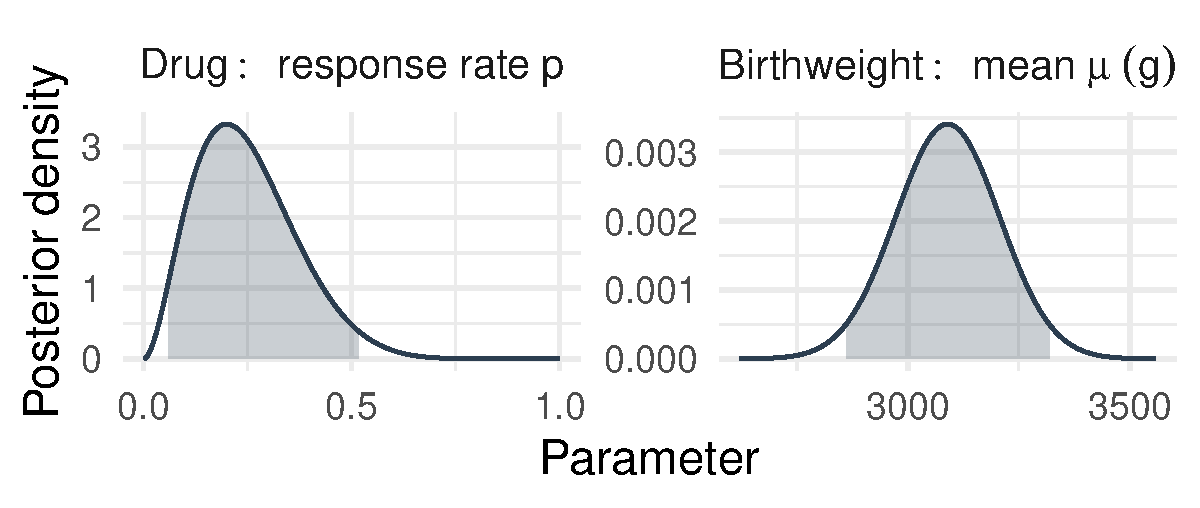
\includegraphics[width=0.86\textwidth]{credible_interval.pdf}
\end{center}

\begin{itemize}
    \item \hl{Drug trial} ($\text{Beta}(3,9)$): $95\%$ CI for $p$ is $[0.06,\; 0.52]$: wide, because $6$ patients is little data.
    \item \hl{Birthweights} ($N(3090, 117^2)$): $95\%$ CI for the mean is $[2860,\; 3319]$\,g, the Lecture 18 value, now with a definition.
\end{itemize}
\end{frame}

%%%%%%%%%%%%%%%%%%%%%%%%%%%%%%%%%%%%%%%%%%%%%%%%%%%%%%%%%%%%%%%%%%%%%%%%
% Section: Hypothesis Testing
%%%%%%%%%%%%%%%%%%%%%%%%%%%%%%%%%%%%%%%%%%%%%%%%%%%%%%%%%%%%%%%%%%%%%%%%
\section{Hypothesis testing}

%%%%%%%%%%%%%%%%%%%%%%%%%%%%%%%%%%%%%%%%%%%%%%%%%%%%%%%%%%%%%%%%%%%%%%%%
\begin{frame}
\frametitle{Testing a hypothesis, Bayesian style}

In Lecture 17, for a discrete event, we answered ``how likely is $H_0$ given the data?'' with the posterior probability itself: $p_{\text{Bayes}} = P(H_0 \mid \text{data})$, and $s_{\text{Bayes}} = -\log_2 p_{\text{Bayes}}$ ``bits of evidence against $H_0$.''

\pause
\medskip

For a \emph{continuous} parameter, a hypothesis is a \hl{region}, and its probability is a \hl{posterior tail area}. Nothing new to invent.

\pause
\medskip

\formula{Bayesian hypothesis test}{$p_{\text{Bayes}} = P(H_0 \mid \text{data})$ \; (a tail area of the posterior), \quad $s_{\text{Bayes}} = -\log_2 p_{\text{Bayes}}$.}
\end{frame}

%%%%%%%%%%%%%%%%%%%%%%%%%%%%%%%%%%%%%%%%%%%%%%%%%%%%%%%%%%%%%%%%%%%%%%%%
\begin{frame}
\frametitle{Two tests, read off the posterior}

\begin{center}
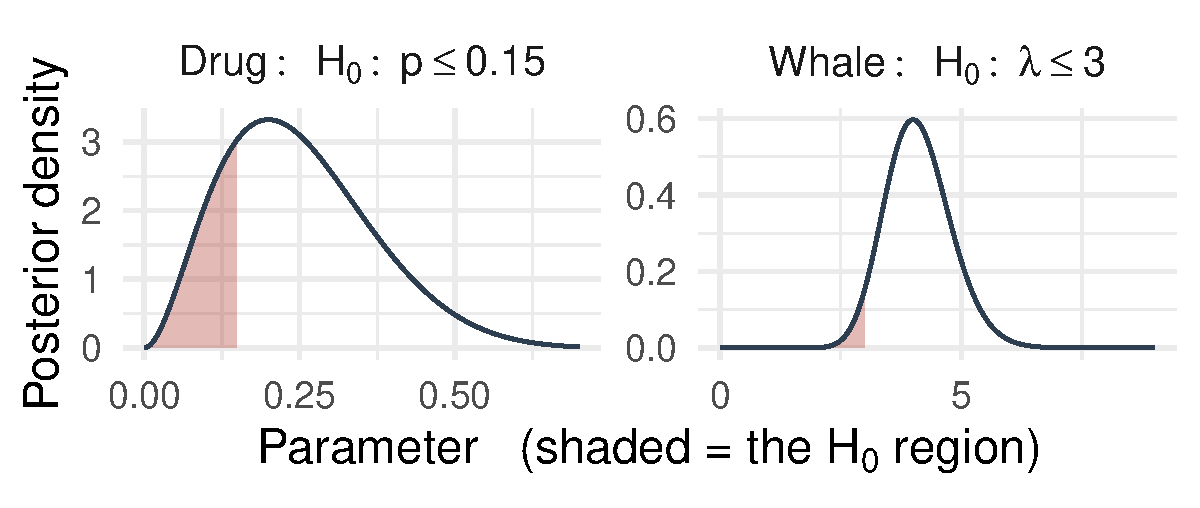
\includegraphics[width=0.8\textwidth]{hypothesis_region.pdf}
\end{center}

\begin{itemize}
    \item \hl{Drug} ($H_0\!: p \le 0.15$): $p_{\text{Bayes}} = 0.22$, so $s_{\text{Bayes}} = 2.2$ bits: modest evidence against $H_0$.
    \item \hl{Whales} ($H_0\!: \lambda \le 3$): $p_{\text{Bayes}} = 0.04$, so $s_{\text{Bayes}} = 4.7$ bits: strong evidence the rate is up.
\end{itemize}
\end{frame}

%%%%%%%%%%%%%%%%%%%%%%%%%%%%%%%%%%%%%%%%%%%%%%%%%%%%%%%%%%%%%%%%%%%%%%%%
\begin{frame}
\frametitle{No null distribution, no $p$-value}

\caution{No null sampling distribution, and no ``assume $H_0$ and see how surprising the data are.'' The whole calculation was: how much posterior probability sits in the $H_0$ region. A larger $s_{\text{Bayes}}$ means more bits of evidence against $H_0$: $2$ bits is a coin landing heads twice, $4.7$ bits nearly five times in a row.}

\pause
\medskip

It is all one idea: \hl{once you have the posterior, every question is an area under it.}
\end{frame}

%%%%%%%%%%%%%%%%%%%%%%%%%%%%%%%%%%%%%%%%%%%%%%%%%%%%%%%%%%%%%%%%%%%%%%%%
% Section: Model Comparison
%%%%%%%%%%%%%%%%%%%%%%%%%%%%%%%%%%%%%%%%%%%%%%%%%%%%%%%%%%%%%%%%%%%%%%%%
\section{Model comparison}

%%%%%%%%%%%%%%%%%%%%%%%%%%%%%%%%%%%%%%%%%%%%%%%%%%%%%%%%%%%%%%%%%%%%%%%%
\begin{frame}
\frametitle{Comparing models, not just parameters}

So far a hypothesis has been a claim about a parameter. But a hypothesis can be a \hl{whole model}. Bayes' rule works exactly the same way:
\[
P(\text{model} \mid \text{data}) \;\propto\; P(\text{model}) \times P(\text{data} \mid \text{model}).
\]
\pause
\medskip

\keyidea{$P(\text{data} \mid \text{model})$ is the probability the model assigned to the data we actually saw, \emph{before} seeing it, averaged over its prior. A prior that is too diffuse, or centered on the wrong values, gives the data a low probability.}

\pause
\medskip

Combine with the prior over models and normalize.
\end{frame}

%%%%%%%%%%%%%%%%%%%%%%%%%%%%%%%%%%%%%%%%%%%%%%%%%%%%%%%%%%%%%%%%%%%%%%%%
\begin{frame}
\frametitle{Which whale model?}
\examplehead{Whale sightings}

Two rival stories for the same $7$ days ($31$ sightings), each equally likely to start:

\smallskip

{\footnotesize
\renewcommand{\arraystretch}{1.2}
\begin{center}
\begin{tabular}{lcccc}
\toprule
\textbf{Model} & \textbf{Prior} & \textbf{Likelihood} & \textbf{Product} & \textbf{Posterior} \\
\midrule
A: baseline $\approx 3$/day & $0.50$ & $0.4596$ & $0.2298$ & $0.31$ \\
B: surge $\approx 5$/day    & $0.50$ & $1.0000$ & $0.5000$ & $\mathbf{0.69}$ \\
\bottomrule
\end{tabular}
\end{center}
}

\smallskip

Multiply across, then divide by the total ($0.2298 + 0.5000 = 0.7298$). The data favor the surge model about $2$ to $1$, but do not \emph{prove} it. (Likelihoods rescaled so the larger reads $1.00$; the rescaling cancels when we normalize.)
\end{frame}

%%%%%%%%%%%%%%%%%%%%%%%%%%%%%%%%%%%%%%%%%%%%%%%%%%%%%%%%%%%%%%%%%%%%%%%%
\begin{frame}
\frametitle{The data re-weight, they don't pick}
\examplehead{Whale sightings}

\begin{center}
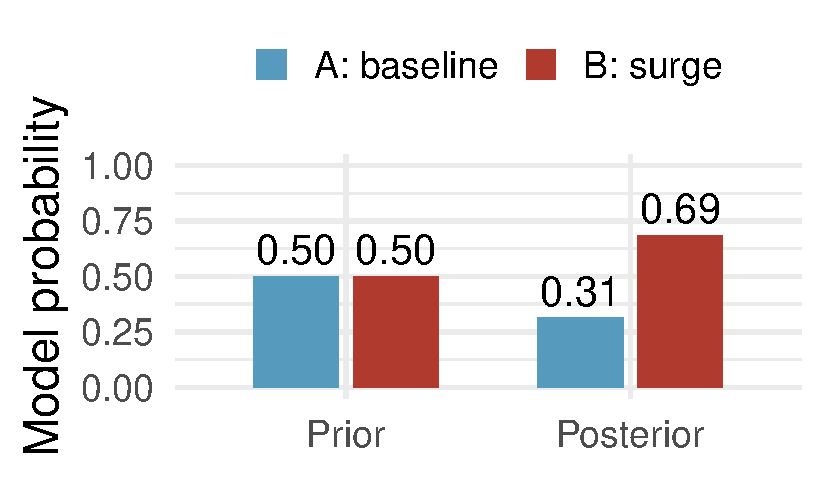
\includegraphics[width=0.55\textwidth]{model_comparison.pdf}
\end{center}

The data did not \emph{pick} a model, they \hl{re-weighted} both. Model B goes from an even bet to roughly a $2$-to-$1$ favorite, and A keeps a third of the probability. With only $7$ days, that is as far as the evidence goes.
\end{frame}

%%%%%%%%%%%%%%%%%%%%%%%%%%%%%%%%%%%%%%%%%%%%%%%%%%%%%%%%%%%%%%%%%%%%%%%%
% Section: Posterior Prediction
%%%%%%%%%%%%%%%%%%%%%%%%%%%%%%%%%%%%%%%%%%%%%%%%%%%%%%%%%%%%%%%%%%%%%%%%
\section{Posterior prediction}

%%%%%%%%%%%%%%%%%%%%%%%%%%%%%%%%%%%%%%%%%%%%%%%%%%%%%%%%%%%%%%%%%%%%%%%%
\begin{frame}
\frametitle{Predicting a new observation: plug-in vs.\ averaging}
\examplehead{Whale sightings}

Given $y_1, \ldots, y_n \sim \text{Poisson}(\lambda)$, predict a new observation $\tilde{y}$.

\pause
\medskip

\hl{Frequentist (plug-in):} estimate $\hat\lambda = \bar{y}$, then predict $\tilde{y} \sim \text{Poisson}(\hat\lambda)$, as if we knew $\lambda$ exactly.

\pause
\medskip

\hl{Bayesian:} we are \emph{not} sure of $\lambda$, so \hl{average} the data model over the posterior:
\formula{Posterior predictive}{$\displaystyle p(\tilde{y} \mid \text{data}) \;\approx\; \frac{1}{M}\sum_{m=1}^{M} p\!\left(\tilde{y} \mid \lambda^{(m)}\right), \qquad \lambda^{(m)} \sim \text{posterior}.$}
\end{frame}

%%%%%%%%%%%%%%%%%%%%%%%%%%%%%%%%%%%%%%%%%%%%%%%%%%%%%%%%%%%%%%%%%%%%%%%%
\begin{frame}
\frametitle{Sampling the posterior predictive}
\examplehead{Whale sightings}

\dq{How do we generate a draw from the posterior predictive?}

\pause
\medskip

Two steps, using the posterior draws we already have (conjugate, grid, or MCMC):
\begin{enumerate}
    \item sample $\lambda^{(m)}$ from the posterior;
    \item sample $\tilde{y}^{(m)} \sim \text{Poisson}\!\left(\lambda^{(m)}\right)$.
\end{enumerate}

\pause
\medskip

Each draw uses a \emph{different} $\lambda$, so the collection $\{\tilde{y}^{(1)}, \ldots, \tilde{y}^{(M)}\}$ carries \hl{both} sources of uncertainty: not knowing $\lambda$, and the randomness of a new count. Swap in any data model and this same recipe works.
\end{frame}

%%%%%%%%%%%%%%%%%%%%%%%%%%%%%%%%%%%%%%%%%%%%%%%%%%%%%%%%%%%%%%%%%%%%%%%%
\begin{frame}
\frametitle{Next day's whale sightings}
\examplehead{Whale sightings}

\begin{center}
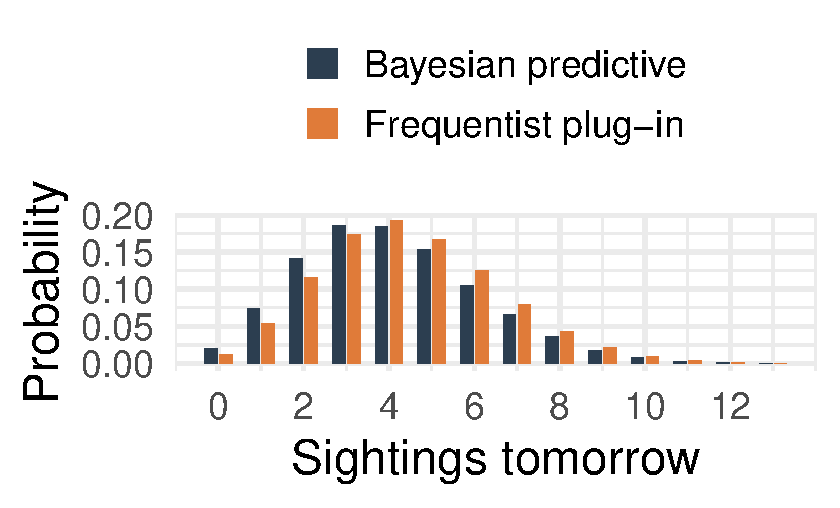
\includegraphics[width=0.56\textwidth]{posterior_predictive_whale.pdf}
\end{center}

\begin{itemize}
    \item Predictive mean $4.1$ (plug-in: $4.4$); $95\%$ interval $[1, 9]$ sightings.
    \item Averaging is \emph{wider in principle}, but $31$ sightings pin $\lambda$ down. The gap grows when data are scarce.
\end{itemize}
\end{frame}

%%%%%%%%%%%%%%%%%%%%%%%%%%%%%%%%%%%%%%%%%%%%%%%%%%%%%%%%%%%%%%%%%%%%%%%%
% Section: Predictive Checking
%%%%%%%%%%%%%%%%%%%%%%%%%%%%%%%%%%%%%%%%%%%%%%%%%%%%%%%%%%%%%%%%%%%%%%%%
\section{Predictive checking}

%%%%%%%%%%%%%%%%%%%%%%%%%%%%%%%%%%%%%%%%%%%%%%%%%%%%%%%%%%%%%%%%%%%%%%%%
\begin{frame}
\frametitle{Is the model any good?}

Every result so far assumes the model is right. But the Poisson model could be wrong, so put it on trial.

\pause
\medskip

\keyidea{\hl{Predictive check:} simulate many replicate datasets from the fitted model, compute a \hl{test statistic} on each, and see where the \emph{observed} value falls. If the real data look like a typical simulation, the model reproduces what matters. If the observed value sits far in the tail, the model is missing something.}

\pause
\medskip

Same posterior-predictive machinery as prediction, but now we simulate whole \emph{datasets}, not a single new point.
\end{frame}

%%%%%%%%%%%%%%%%%%%%%%%%%%%%%%%%%%%%%%%%%%%%%%%%%%%%%%%%%%%%%%%%%%%%%%%%
\begin{frame}
\frametitle{Checking the whale model}
\examplehead{Whale sightings}

\vspace{1.4em}

\twocol{0.5}{0.5}{
Simulate $5000$ replicate weeks; the statistic is the \hl{busiest day's count} (observed $=7$). The \hl{predictive $p$-value} is the fraction at least as extreme: $P(T_{\text{rep}} \ge 7) = 0.57$, right in the bulk, so \hl{no reason to doubt} the Poisson fit.

\medskip

\hl{Careful:} not the $p_{\text{Bayes}}$ of a hypothesis test. There \emph{small} meant evidence against $H_0$; here the \hl{middle is good}.
}{
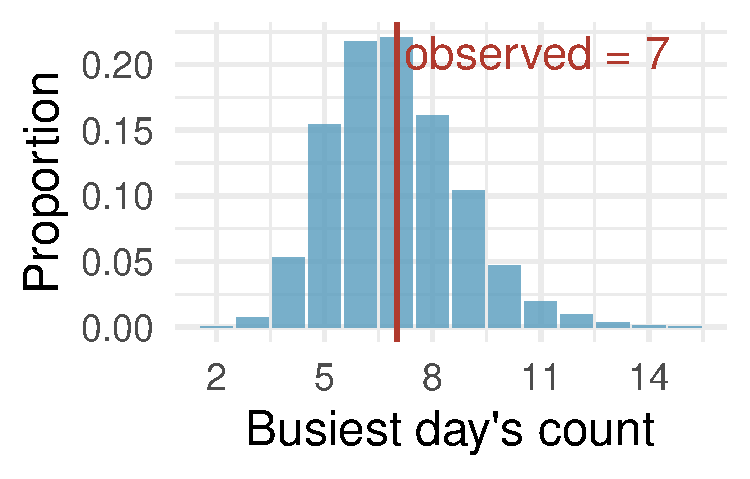
\includegraphics[width=\textwidth]{predictive_check.pdf}
}
\end{frame}

%%%%%%%%%%%%%%%%%%%%%%%%%%%%%%%%%%%%%%%%%%%%%%%%%%%%%%%%%%%%%%%%%%%%%%%%
% Section: Wrap-up
%%%%%%%%%%%%%%%%%%%%%%%%%%%%%%%%%%%%%%%%%%%%%%%%%%%%%%%%%%%%%%%%%%%%%%%%
\section{Wrap-up}

%%%%%%%%%%%%%%%%%%%%%%%%%%%%%%%%%%%%%%%%%%%%%%%%%%%%%%%%%%%%%%%%%%%%%%%%
\begin{frame}
\frametitle{Summary}

Once you have the posterior, inference is just \emph{reading} it:
{\small
\begin{itemize}
    \item \hl{Point estimate:} the posterior mean, shrunk from the MLE toward the prior.
    \pause
    \item \hl{Credible interval:} the central $95\%$ of the posterior, $P(a \le \theta \le b \mid \text{data}) = 0.95$.
    \pause
    \item \hl{Hypothesis test:} the posterior probability of the $H_0$ region, reported as $s_{\text{Bayes}} = -\log_2 p_{\text{Bayes}}$ bits.
    \pause
    \item \hl{Model comparison:} Bayes' rule over models rather than parameters.
    \pause
    \item \hl{Prediction:} average the data model over the posterior, carrying both kinds of uncertainty.
    \pause
    \item \hl{Predictive checking:} simulate replicate data and compare a test statistic to the observed one.
\end{itemize}}
\end{frame}

%%%%%%%%%%%%%%%%%%%%%%%%%%%%%%%%%%%%%%%%%%%%%%%%%%%%%%%%%%%%%%%%%%%%%%%%
\begin{frame}
\frametitle{Frequentist $\longleftrightarrow$ Bayesian: a summary}

Every task today had a frequentist counterpart you already know:

{\footnotesize
\renewcommand{\arraystretch}{1.25}
\begin{center}
\begin{tabular}{p{2.2cm} p{2.9cm} p{3.4cm}}
\toprule
\textbf{Task} & \textbf{Frequentist} & \textbf{Bayesian} \\
\midrule
Point estimate & MLE $\hat\theta$ & Posterior mean \\
Interval & Confidence interval & Credible interval \\
Hypothesis & $p$-value & $P(H_0 \mid \text{data})$ \\
New observation & Prediction interval & Posterior predictive \\
Computation & Formulas / bootstrap & Conjugate / grid / MCMC \\
\bottomrule
\end{tabular}
\end{center}
}

\pause

With plenty of data the two usually agree. The differences show up with \hl{small samples} or an \hl{informative prior}, which is exactly where the prior still matters.
\end{frame}

%%%%%%%%%%%%%%%%%%%%%%%%%%%%%%%%%%%%%%%%%%%%%%%%%%%%%%%%%%%%%%%%%%%%%%%%
\begin{frame}
\frametitle{Coming up next}

\hl{We can now compute a posterior and read every kind of inference off it}, for one parameter or a handful.

\vspace{0.4em}
\begin{itemize}
\item \hl{Lecture 21: Bayesian linear regression.} We put a whole \emph{regression} model into the Bayesian frame: a slope, an intercept, and noise, each with its own prior.
\pause
\item The new question is \hl{how to choose priors for the coefficients}: vague where we know nothing, informative where we do. Everything from today (credible intervals for the slope, prediction for a new case) then carries over unchanged.
\end{itemize}
\end{frame}

%%%%%%%%%%%%%%%%%%%%%%%%%%%%%%%%%%%%%%%%%%%%%%%%%%%%%%%%%%%%%%%%%%%%%%%%
% Activity Frame
%%%%%%%%%%%%%%%%%%%%%%%%%%%%%%%%%%%%%%%%%%%%%%%%%%%%%%%%%%%%%%%%%%%%%%%%
\begin{frame}
\frametitle{In-class activity}

You'll work in \textbf{pairs} (one analyst, one guide).

\medskip
\begin{itemize}
\item Pick up the worksheet.
\item Work through the problems together.
\item \hl{Don't use Gen AI except for debugging}
\item Your worksheet will be collected and graded.
\end{itemize}

\medskip
\textbf{Recommendations:}
\begin{itemize}
\item Read each question carefully before starting the code.
\item Discuss your answers with your partner before writing them down.
\end{itemize}

\end{frame}

\end{document}
